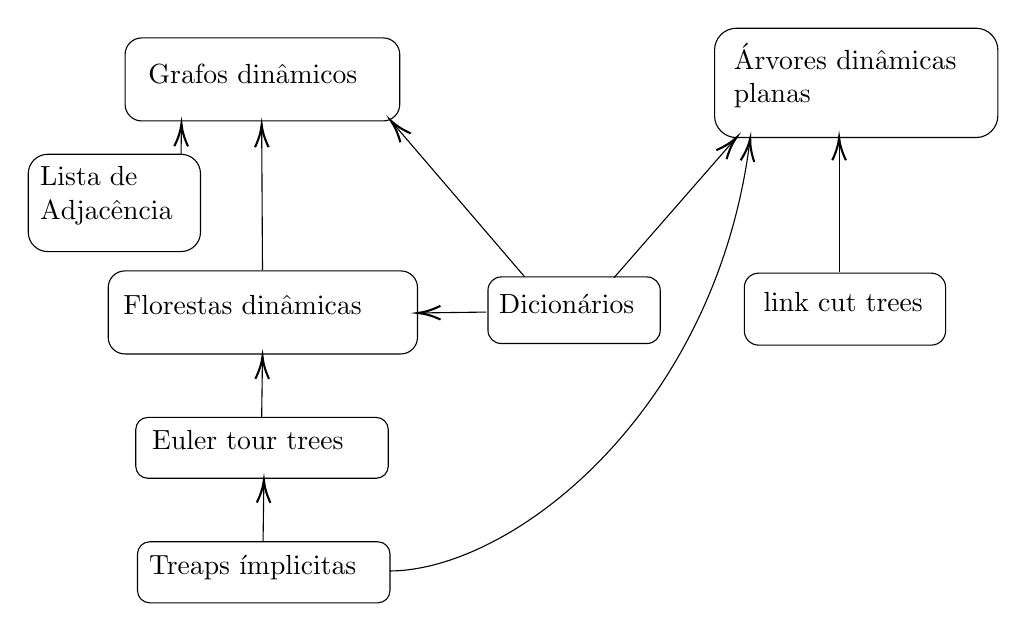
\begin{tikzpicture}[x=0.75pt,y=0.75pt,yscale=-1,xscale=1]
%uncomment if require: \path (0,390); %set diagram left start at 0, and has height of 390

%Rounded Rect [id:dp5638261819516392] 
\draw   (89.47,271.31) .. controls (89.47,268.07) and (92.1,265.43) .. (95.35,265.43) -- (205.25,265.43) .. controls (208.5,265.43) and (211.13,268.07) .. (211.13,271.31) -- (211.13,288.95) .. controls (211.13,292.2) and (208.5,294.83) .. (205.25,294.83) -- (95.35,294.83) .. controls (92.1,294.83) and (89.47,292.2) .. (89.47,288.95) -- cycle ;
%Rounded Rect [id:dp9959376432936062] 
\draw   (75.37,142.93) .. controls (75.37,138.52) and (78.95,134.93) .. (83.37,134.93) -- (216.37,134.93) .. controls (220.78,134.93) and (224.37,138.52) .. (224.37,142.93) -- (224.37,166.93) .. controls (224.37,171.35) and (220.78,174.93) .. (216.37,174.93) -- (83.37,174.93) .. controls (78.95,174.93) and (75.37,171.35) .. (75.37,166.93) -- cycle ;
%Rounded Rect [id:dp7099894103599613] 
\draw   (83.5,30.67) .. controls (83.5,26.25) and (87.08,22.67) .. (91.5,22.67) -- (207.83,22.67) .. controls (212.25,22.67) and (215.83,26.25) .. (215.83,30.67) -- (215.83,54.67) .. controls (215.83,59.08) and (212.25,62.67) .. (207.83,62.67) -- (91.5,62.67) .. controls (87.08,62.67) and (83.5,59.08) .. (83.5,54.67) -- cycle ;
%Rounded Rect [id:dp9694794812846669] 
\draw   (258.33,144.25) .. controls (258.33,140.7) and (261.2,137.83) .. (264.75,137.83) -- (334.92,137.83) .. controls (338.46,137.83) and (341.33,140.7) .. (341.33,144.25) -- (341.33,163.49) .. controls (341.33,167.03) and (338.46,169.9) .. (334.92,169.9) -- (264.75,169.9) .. controls (261.2,169.9) and (258.33,167.03) .. (258.33,163.49) -- cycle ;
%Rounded Rect [id:dp08232296692986518] 
\draw   (381.83,142.93) .. controls (381.83,139.1) and (384.94,136) .. (388.77,136) -- (471.9,136) .. controls (475.73,136) and (478.83,139.1) .. (478.83,142.93) -- (478.83,163.73) .. controls (478.83,167.56) and (475.73,170.67) .. (471.9,170.67) -- (388.77,170.67) .. controls (384.94,170.67) and (381.83,167.56) .. (381.83,163.73) -- cycle ;
%Rounded Rect [id:dp3985250366724754] 
\draw   (367.5,28.53) .. controls (367.5,22.72) and (372.22,18) .. (378.03,18) -- (493.47,18) .. controls (499.28,18) and (504,22.72) .. (504,28.53) -- (504,60.13) .. controls (504,65.95) and (499.28,70.67) .. (493.47,70.67) -- (378.03,70.67) .. controls (372.22,70.67) and (367.5,65.95) .. (367.5,60.13) -- cycle ;
%Straight Lines [id:da5589289981455373] 
\draw    (149.7,134.4) -- (149.31,66.4) ;
\draw [shift={(149.3,64.4)}, rotate = 89.67] [color={rgb, 255:red, 0; green, 0; blue, 0 }  ][line width=0.75]    (10.93,-3.29) .. controls (6.95,-1.4) and (3.31,-0.3) .. (0,0) .. controls (3.31,0.3) and (6.95,1.4) .. (10.93,3.29)   ;
%Straight Lines [id:da8087039160610074] 
\draw    (149.3,205.6) -- (149.67,178) ;
\draw [shift={(149.7,176)}, rotate = 90.77] [color={rgb, 255:red, 0; green, 0; blue, 0 }  ][line width=0.75]    (10.93,-3.29) .. controls (6.95,-1.4) and (3.31,-0.3) .. (0,0) .. controls (3.31,0.3) and (6.95,1.4) .. (10.93,3.29)   ;
%Straight Lines [id:da19920966114360028] 
\draw    (257.5,154.75) -- (226.5,155.17) ;
\draw [shift={(224.5,155.2)}, rotate = 359.22] [color={rgb, 255:red, 0; green, 0; blue, 0 }  ][line width=0.75]    (10.93,-3.29) .. controls (6.95,-1.4) and (3.31,-0.3) .. (0,0) .. controls (3.31,0.3) and (6.95,1.4) .. (10.93,3.29)   ;
%Straight Lines [id:da38139604958901885] 
\draw    (319,138.25) -- (376.72,72.17) ;
\draw [shift={(378.03,70.67)}, rotate = 131.14] [color={rgb, 255:red, 0; green, 0; blue, 0 }  ][line width=0.75]    (10.93,-3.29) .. controls (6.95,-1.4) and (3.31,-0.3) .. (0,0) .. controls (3.31,0.3) and (6.95,1.4) .. (10.93,3.29)   ;
%Straight Lines [id:da5633794503104798] 
\draw    (427.5,135.33) -- (427.5,72.67) ;
\draw [shift={(427.5,70.67)}, rotate = 90] [color={rgb, 255:red, 0; green, 0; blue, 0 }  ][line width=0.75]    (10.93,-3.29) .. controls (6.95,-1.4) and (3.31,-0.3) .. (0,0) .. controls (3.31,0.3) and (6.95,1.4) .. (10.93,3.29)   ;
%Straight Lines [id:da7918857844120134] 
\draw    (276,137.75) -- (212.8,64.02) ;
\draw [shift={(211.5,62.5)}, rotate = 49.4] [color={rgb, 255:red, 0; green, 0; blue, 0 }  ][line width=0.75]    (10.93,-3.29) .. controls (6.95,-1.4) and (3.31,-0.3) .. (0,0) .. controls (3.31,0.3) and (6.95,1.4) .. (10.93,3.29)   ;
%Rounded Rect [id:dp21131335155672382] 
\draw   (36.83,88.11) .. controls (36.83,82.93) and (41.03,78.73) .. (46.21,78.73) -- (110.46,78.73) .. controls (115.64,78.73) and (119.83,82.93) .. (119.83,88.11) -- (119.83,116.23) .. controls (119.83,121.4) and (115.64,125.6) .. (110.46,125.6) -- (46.21,125.6) .. controls (41.03,125.6) and (36.83,121.4) .. (36.83,116.23) -- cycle ;
%Straight Lines [id:da7631806191728931] 
\draw    (110.46,78.73) -- (110.63,65.93) ;
\draw [shift={(110.66,63.93)}, rotate = 90.77] [color={rgb, 255:red, 0; green, 0; blue, 0 }  ][line width=0.75]    (10.93,-3.29) .. controls (6.95,-1.4) and (3.31,-0.3) .. (0,0) .. controls (3.31,0.3) and (6.95,1.4) .. (10.93,3.29)   ;
%Curve Lines [id:da8410667922534024] 
\draw    (211,279.5) .. controls (270.37,279.17) and (367.69,202.93) .. (384.42,73.13) ;
\draw [shift={(384.67,71.17)}, rotate = 96.96] [color={rgb, 255:red, 0; green, 0; blue, 0 }  ][line width=0.75]    (10.93,-3.29) .. controls (6.95,-1.4) and (3.31,-0.3) .. (0,0) .. controls (3.31,0.3) and (6.95,1.4) .. (10.93,3.29)   ;
%Rounded Rect [id:dp3745338241823657] 
\draw   (88.63,211.37) .. controls (88.63,208.13) and (91.26,205.5) .. (94.5,205.5) -- (204.43,205.5) .. controls (207.67,205.5) and (210.3,208.13) .. (210.3,211.37) -- (210.3,228.97) .. controls (210.3,232.21) and (207.67,234.83) .. (204.43,234.83) -- (94.5,234.83) .. controls (91.26,234.83) and (88.63,232.21) .. (88.63,228.97) -- cycle ;
%Straight Lines [id:da6552331155919412] 
\draw    (149.97,265.27) -- (150.34,237.67) ;
\draw [shift={(150.37,235.67)}, rotate = 90.77] [color={rgb, 255:red, 0; green, 0; blue, 0 }  ][line width=0.75]    (10.93,-3.29) .. controls (6.95,-1.4) and (3.31,-0.3) .. (0,0) .. controls (3.31,0.3) and (6.95,1.4) .. (10.93,3.29)   ;

% Text Node
\draw (93.8,270.43) node [anchor=north west][inner sep=0.75pt]   [align=left] {Treaps ímplicitas};
% Text Node
\draw (81.37,145.6) node [anchor=north west][inner sep=0.75pt]   [align=left] {Florestas dinâmicas};
% Text Node
\draw (93.5,34.33) node [anchor=north west][inner sep=0.75pt]   [align=left] {Grafos dinâmicos};
% Text Node
\draw (262.5,145) node [anchor=north west][inner sep=0.75pt]   [align=left] {Dicionários};
% Text Node
\draw (389.83,144) node [anchor=north west][inner sep=0.75pt]   [align=left] {link cut trees};
% Text Node
\draw (375.5,24) node [anchor=north west][inner sep=0.75pt]   [align=left] {Árvores dinâmicas\\planas};
% Text Node
\draw (41.3,83.4) node [anchor=north west][inner sep=0.75pt]   [align=left] {Lista de\\Adjacência};
% Text Node
\draw (95.3,210.5) node [anchor=north west][inner sep=0.75pt]   [align=left] {Euler tour trees};
\end{tikzpicture}
